\subsection{RQ3 --- Do explanations stay the same when the network changes?}
\label{sec:rq3}
We compared the top-5 features of the four attack families shared by CIC-IDS2017 and CSE-CIC-IDS2018 (Fig.~\ref{fig:drift}).
\begin{itemize}[leftmargin=*, itemsep=0pt]
  \item \textbf{Within one network, explanations are stable:} two random halves of the data agree 0.99 (Jaccard@5), and a model retrained with another seed still agrees 0.82. They also stay stable over time.
  \item \textbf{Across networks they change:} agreement falls to 0.48 when the same model is used on the other network, and to 0.17 when each network has its own model. That is below both noise levels in 12 of 16 cases.
  \item \textbf{The change follows the accuracy loss} (Spearman $\rho=0.63$, $p=0.008$). For DoS, recall falls from 0.94 to 0.43 and top-5 agreement to 0.43, so the model shows confident but outdated reasons for exactly the flows it now misses.
  \item \textbf{Transfer costs 20--34 F1 points.} Hiding ports and headers ($T_3$) lowers the false-positive rate after the change (9.9--11.9\% instead of 16.8--19.4\% on $T_1$).
\end{itemize}
H3 is supported: watching explanation drift can warn of a network change before labelled data are available.

\begin{figure}[!htbp]
\centering
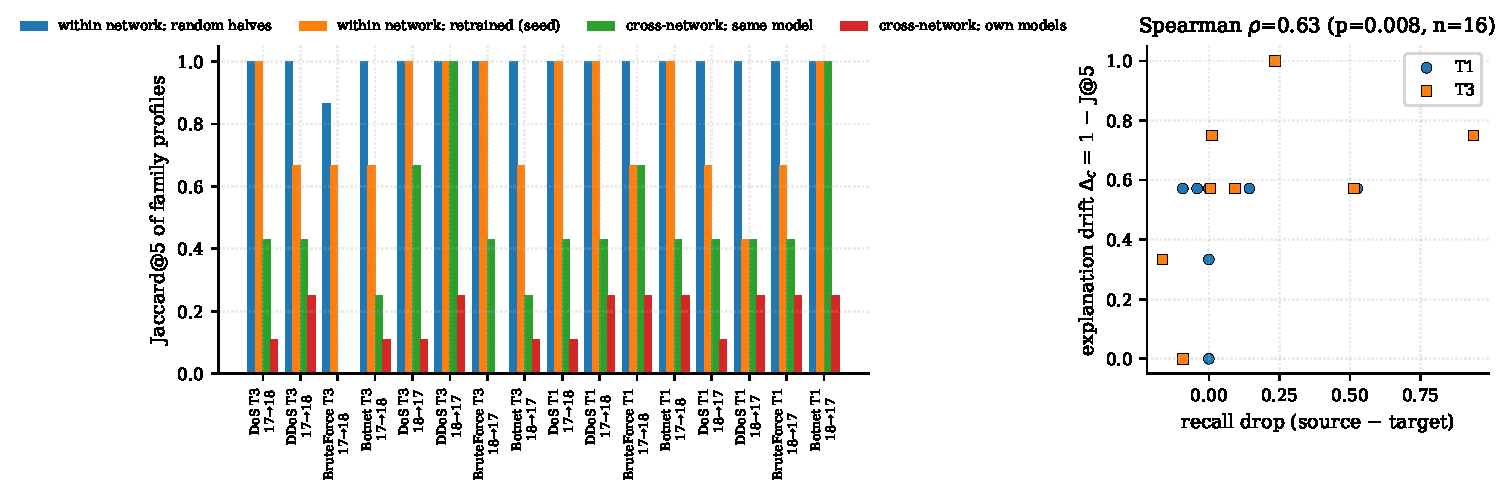
\includegraphics[width=0.9\textwidth]{../figures/fig_drift.pdf}
\caption{Left: top-5 agreement of attack-family explanations within one network (two noise levels) and across networks. Right: explanation drift against the drop in recall for the same family.}
\label{fig:drift}
\end{figure}
